\documentclass[12pt, a4paper]{report}
\usepackage[top=1.0in, bottom=1.0in, left=0.8in, right=0.8in]{geometry}
\usepackage{graphicx}
\usepackage{amsmath}
\usepackage{listings}
\usepackage{fancyvrb}

 	
\title{\textbf{EE2703 : Applied Programming Lab \\ Assignment 9\\Spectra of non-periodic signals }} 
\author{Aditya Nanda Kishore\\ EE20B062} 

\date{\today} % Date for the report

	
\begin{document}
		
\maketitle
\section*{Introduction}
In the previous assignment we looked at functions that were periodic and extracted their spectra.Now we want to look at non-periodic signals.In this Assignment, 
\begin{itemize}
\item We will understand what should be the sampling frequency and sampling length for non periodic signals for obtaining their DFT
\item We will see how the use of windowing functions (e.g \textbf{Hamming Window}) can help in making the DFT better.
\item We will explore DFT without and with windowing. Windowing is used to make the signal integrable and it reduces the discontinuities in the actual signal that can lead to inaccurate DFTs 
\item We will learn how to estimate $\omega_0$(Frequency of signal in time domain) and $\delta$(Initial phase of the system in time domain) from DFT in absence and presence of noise
\end{itemize}

\section*{Libraries and Spectrum Function}
Just like that of in the previous assignment, we are going to use a spectrum function to call and plot spectra of different functions.The code is given below.
\par\noindent\rule{\textwidth}{0.4pt}
\begin{Verbatim}
def spectrum(func,T,t_0,time_check, N, windowing, xlim,plot, plot_name, fig_name):
    if (time_check):
        t = np.linspace(-T,T, N+1)[:-1]
    elif (time_check == False):
        t = t_0
    dt=t[1]-t[0];fmax=1/dt
    y= func(t)
    y[0]=0
    if (windowing) :
        n=np.arange(N)
        wnd=np.fft.fftshift(0.54+0.46*np.cos(2*np.pi*n/(N-1)))
        y = y*wnd

    y=np.fft.fftshift(y) # make y start with y(t=0)
    Y=np.fft.fftshift(np.fft.fft(y))/N
    w=np.linspace(-np.pi*fmax,np.pi*fmax,N+1);w=w[:-1]
    if (plot):
        plt.figure()
        plt.subplot(2,1,1)
        plt.plot(w,abs(Y), lw = 2)
        plt.xlim([-xlim, xlim])
        plt.ylabel(r"$|Y|$",size=16)
        plt.title(plot_name)
        plt.grid(True)
        plt.subplot(2,1,2)
        np.angle(Y)[np.where(np.abs(Y)<3e-3)] = 0
        plt.plot(w,np.angle(Y),'ro',lw=2)
        plt.xlim([-xlim, xlim])
        plt.ylabel(r"Phase of $Y$",size=16)
        plt.xlabel(r"$k$",size=16)
        plt.grid(True)
        plt.savefig(fig_name)
        plt.show()
    return Y,w
   \end{Verbatim}
   \par\noindent\rule{\textwidth}{0.4pt}
   
 \section*{Example - DFT of $sin(\sqrt{2}t)$} 
 \small
 \subsection*{Without Windowing}
 \normalsize
 
 We will first plot the DFT of  $sin(\sqrt{2}t)$ normally by taking $t$'s limits as $[-\pi,\pi)$, $\omega$'s limits as $ [-\pi f_{max}, \pi f_{max})$, $N  = 64$ and setting the first value of function array to zero.
 
 \begin{Verbatim}
#Examples
t_0 = np.zeros(64)

def sinsqrt(t, w0 = np.sqrt(2)):
    return(np.sin(t*w0))
#Without Hamming

spectrum(sinsqrt,np.pi, t_0,True, 64, False, 10, True,"
Spectrum of $sin(\sqrt{2}t)$", "Q1a.png")
   \end{Verbatim}

  \begin{figure}[!tbh]
   	\centering
   	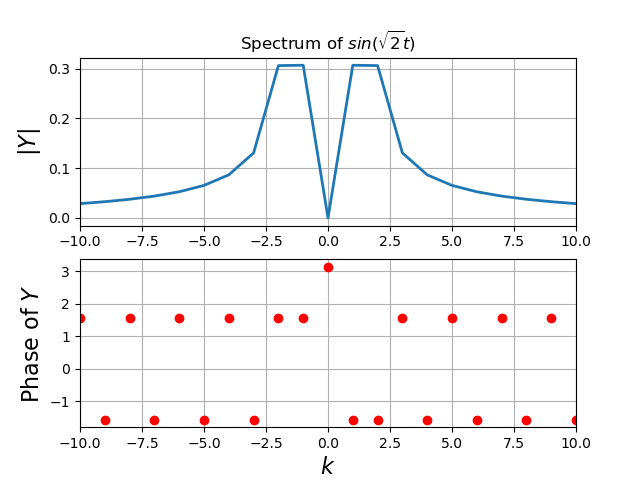
\includegraphics[scale=0.7]{Q1a.png}
	\caption{Spectrum of $sin(\sqrt{2}t)$ without hamming}
 \end{figure} 
 We expected two spikes, but what we got were two peaks each with two values and a gradually decaying magnitude
  \subsection*{With Windowing}
 Well the spikes happen at the end of the periodic interval. So we damp the function near there, i.e., we multiply our function sequence f [n] by a “window” sequence w[n]:
 \begin{equation*}
w(n) =  \left\{
        \begin{array}{ll}
            0.54+0.46cos(\frac{2\pi n}{N-1}) & \quad |n| \leq \frac{N-1}{2} \\
           0& \quad else      
             \end{array}
    \right.
 \end{equation*}
 
 \begin{Verbatim}
spectrum(sinsqrt,np.pi,t_0,True, 64, True, 10, True,
 "Spectrum of $sin(\sqrt{2}t)$, with Windowing", "Q1b.png")

spectrum(sinsqrt,4*np.pi,t_0,True, 128, True, 10, True, 
"Improved Spectrum of $sin(\sqrt{2}t)$, with Windowing", "Q1c.png")  
 \end{Verbatim}

 \begin{figure}[!tbh]
   	\centering
   	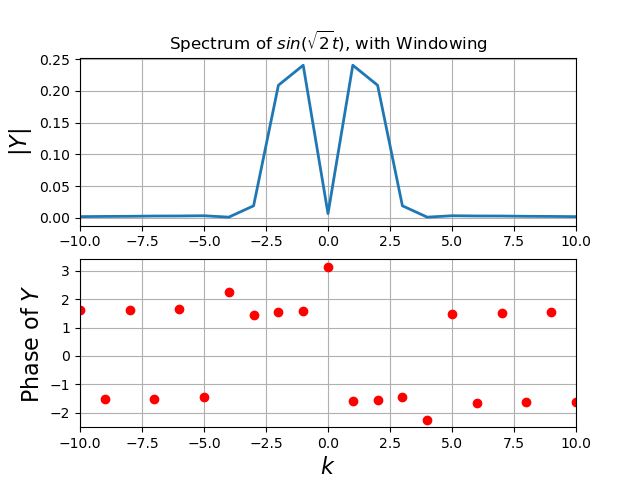
\includegraphics[scale=0.7]{Q1b.png}
	\caption{Spectrum of $sin(\sqrt{2}t)$ with windowing}
 \end{figure} 
  \begin{figure}[!tbh]
   	\centering
   	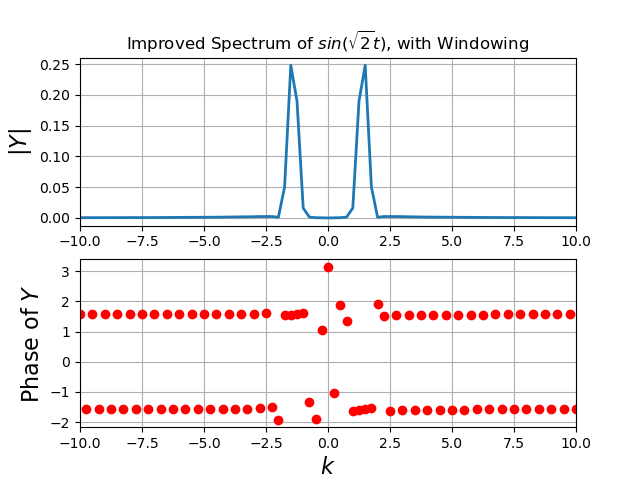
\includegraphics[scale=0.7]{Q1c.png}
	\caption{Improved Spectrum of $sin(\sqrt{2}t)$ with windowing}
 \end{figure} 
\newpage
 \section*{DFT of $cos^3(\omega_0t)$} 
   Consider the function $cos^3(\omega_0t)$. We are going to obtain its spectrum for $\omega_0$ = 0.86 with and without a hamming window.
 \small

 \subsection*{Without Windowing}
 
 \normalsize
  \begin{Verbatim}
#Question 2

def cos3(t,w0=0.86):
    return (np.cos(w0*t))**3

#Without Hamming

spectrum(cos3,4*np.pi,t_0,True, 64, False, 5, True,"
Spectrum of $cos^3(0.86t)$", "Q2a.png")
\end{Verbatim}

 \begin{figure}[!tbh]
   	\centering
   	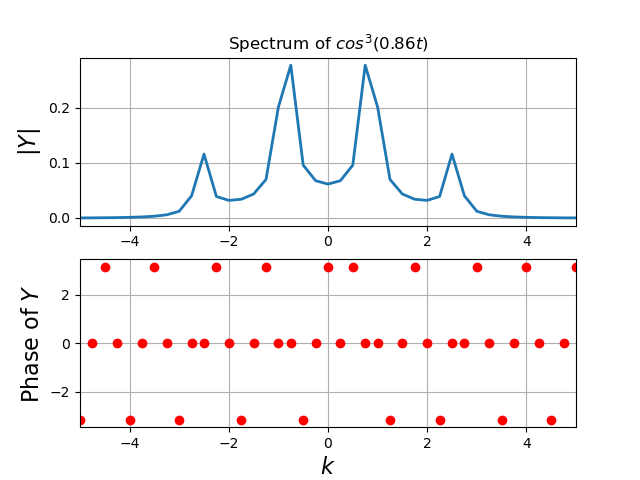
\includegraphics[scale=0.7]{Q2a.png}
	\caption{Spectrum of $cos^3(0.86t)$ without windowing}
 \end{figure} 
 

  \subsection*{With Windowing}
 
 \normalsize
  \begin{Verbatim}
spectrum(cos3,4*np.pi,t_0,True, 64, True, 5, True, 
"Spectrum of $cos^3(0.86t)$, with windowing ", "Q2b.png")
\end{Verbatim}
 
 
 
 
  \begin{figure}[!tbh]
   	\centering
   	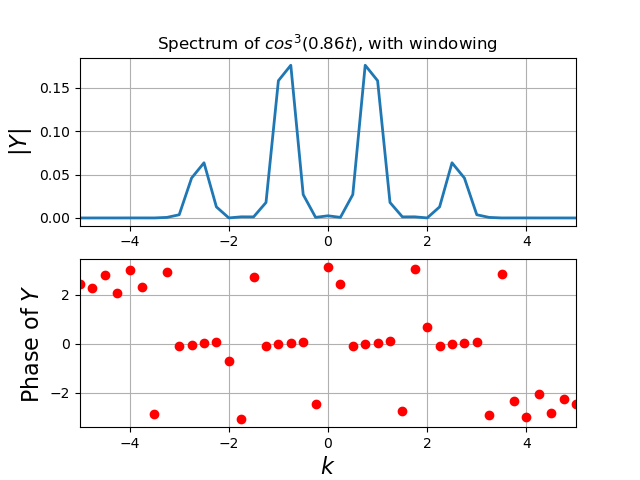
\includegraphics[scale=0.7]{Q2b.png}
	\caption{Spectrum of $cos^3(0.86t)$ with windowing}
 \end{figure} 

From the plots, we can see that hamming has improved the accuracy of both phase and magnitude of the DFT spectrum

 \section*{Statistical Estimation of $\delta$ and $\omega_0$ } 
 
 After the spectra is obtained, the resolution is not enough to obtain the $omega_0$ directly. The peaks will cannot be obtained as the sampling frequency is not enough to cover all the omegas, so we might the peak value actually. So a statistical estimation of $\omega_0$ is necessary. Hence, we can obtain $\omega_0$ by taking a weighted average of all the $\omega_0$ weighted with the squared magnitude of the DFT or we can also take the mean, with the former as more accurate version
 
 \begin{equation*}
 \omega_0 = \frac{\sum_{} ^{} \omega_i |Y(\omega_i)|^2}{ |Y(\omega_i)|^2}   
  \end{equation*}
 
  Similarly, delta can be obtained using the phase of the discrete fourier transform at $\omega_0$ nearest to estimated $\omega$.The python code snippet to carry out the above is as follows.I took $\omega_0= 1.5$ and $\delta = 0.5$ for calculations as these two numbers are not close the sampled frequencies.The Plots and the values I got are,I windowed it for more accuracy
  
    \begin{Verbatim}
def cos(t,w0 = 1, delta = 0.8):
    return(np.cos(w0*t+delta))

Y,w=spectrum(cos,np.pi, t_0,True,128, True, 5, True,
"Spectrum of $cos(1t+0.8)$", "Q3.png")

ii = np.where(w>0)
omega = (sum(abs(Y[ii])**2*w[ii])/sum(abs(Y[ii])**2))
print ("omega_0 = ", omega)

i = abs(w-omega).argmin()
delta = np.angle(Y[i])
print ("delta = ", delta)
\end{Verbatim}
 
   \begin{figure}[!tbh]
   	\centering
   	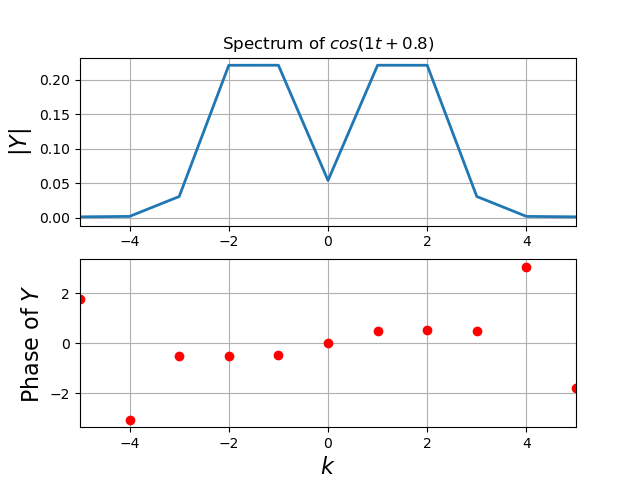
\includegraphics[scale=0.7]{Q3.png}
	\caption{Spectrum of $cos(1.5t+0.5)$ with windowing}
 \end{figure} 

Calculated Values are
\begin{itemize}

      \item $\omega_0$ =  1.5170146006408245
      \item $\delta =  0.5185215763925791$ 
\end{itemize}
   
   
  \section*{Statistical Estimation of $\delta$ and $\omega_0$ in presence of noise} 
  We go on with defining a noisy cosine function generated by adding white guassian noise(\textbf{randn} function)with same $\omega_0$ and $\delta$ as above and estimate them using same set of equations.The code and plots, results obtained are
  
    
    \begin{Verbatim}
def noisycos(t,w0 = 1.5, delta = 0.5):
    return(np.cos(w0*t+delta)+0.1*np.random.randn(128))

Y,w=spectrum(noisycos,np.pi,t_0,True, 128, True, 5, True,
 "Spectrum of Noisy $cos(1t+0.8)$", "Q4.png")

ii = np.where(w > 0)
omega = (sum(abs(Y[ii])**2*w[ii])/sum(abs(Y[ii])**2))
print ("noisy signal's omega_0 = ", omega)

i = abs(w-omega).argmin()
delta = np.angle(Y[i])
print ("noisy signal's delta = ", delta)
\end{Verbatim}
 
   \begin{figure}[!tbh]
   	\centering
   	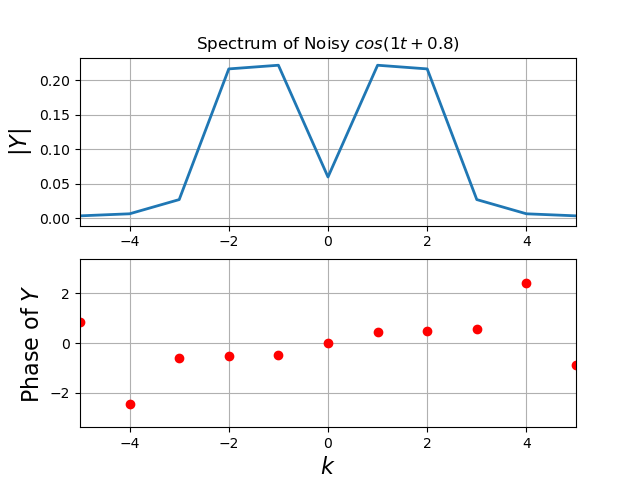
\includegraphics[scale=0.7]{Q4.png}
	\caption{Spectrum of Noisy $cos(1.5t+0.5)$ with windowing}
 \end{figure} 

Calculated Values are
\begin{itemize}

      \item $\omega_0$ =  1.7504472605048746
      \item $\delta =  0.8126378047378449$ 
      \item This error is slightly higher compared to the case without noise

\end{itemize}
   
  \section*{Chirped Signal Spectrum} 
  Consider a chirped signal, $cos(16(1.5t+ \frac{t^2}{2\pi}))$ where t $\epsilon   [-\pi,\pi)$. Its frequency continuously changes from 16 to 32 radians per second. This also means that the period is 64 samples near $-\pi$ and is 32 samples near $\pi$. The DFT plot for this signal is as follows
  \begin{Verbatim}
  
def chirp(t):
    return (np.cos(24*t+ 16*(t**2)/(2*np.pi)))
spectrum(chirp,np.pi, t_0, True,1024, True, 100, True,
"Spectrum of Chirped Signal", "Q5.png")
\end{Verbatim}

   \begin{figure}[!tbh]
   	\centering
   	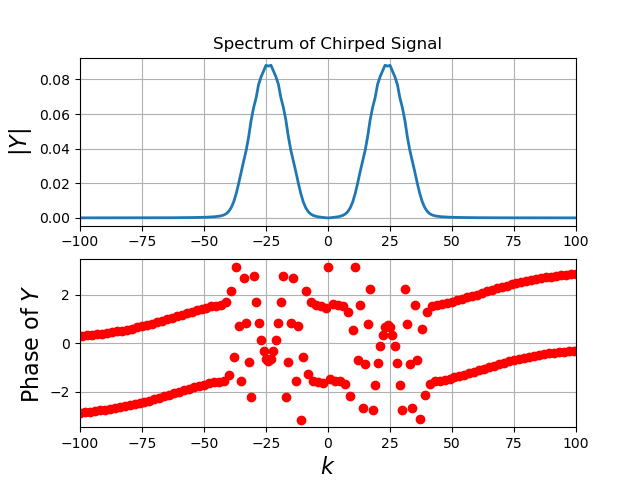
\includegraphics[scale=0.7]{Q5.png}
	\caption{Spectrum of chirp signal with windowing}
 \end{figure} 

\section*{Surface plot of chirped signal}
We now break the same chirped signal's 1024 vector into pieces that are 64 samples wide. Extract the DFT of each and store as a column in a 2D array.Then plot the array as a surface plot to show how the frequency of the signal varies with time.Plot and analyse the time frequency plot.This is a “time- frequency” plot, where we get localized DFTs and show how the spectrum evolves in time.

\footnotesize

\begin{Verbatim}
t=np.linspace(-np.pi,np.pi,1025);t=t[:-1]
t_arrays=np.split(t,16)

Y_mag=np.zeros((16,64))
Y_phase=np.zeros((16,64))


for i in range(len(t_arrays)):
    Y,w = spectrum(chirp, np.pi, t_arrays[i], False, 64,False, 60, False,"Spectrum of Chirp Function", "Q5.png")
    Y_mag[i] = np.abs(Y)
    Y_phase[i] = np.angle(Y)

fig = plt.figure()
ax = fig.add_subplot(111, projection='3d')

t=np.linspace(-np.pi,np.pi,1025);t=t[:-1]
fmax = 1/(t[1]-t[0])
t=t[::64]
w=np.linspace(-fmax*np.pi,fmax*np.pi,64+1);w=w[:-1]
t,w=np.meshgrid(t,w)

surf=ax.plot_surface(w,t,Y_mag.T,cmap=plt.cm.coolwarm,linewidth=0, antialiased=False)
fig.colorbar(surf, shrink=0.5, aspect=5)
plt.ylabel("Frequency")
plt.xlabel("Time")
plt.title("Surface Plot- Magnitude")
plt.savefig("Q6a.png")
plt.show()

fig = plt.figure()
ax = fig.add_subplot(111, projection='3d')
surf=ax.plot_surface(w,t,Y_phase.T,cmap=plt.cm.coolwarm,linewidth=0, antialiased=False)
fig.colorbar(surf, shrink=0.5, aspect=5)
plt.ylabel("Frequency")
plt.xlabel("Time")
plt.title("Surface Plot-Phase")
plt.savefig("Q6b.png")
plt.show()


\end{Verbatim}

    \begin{figure}[!tbh]
   	\centering
   	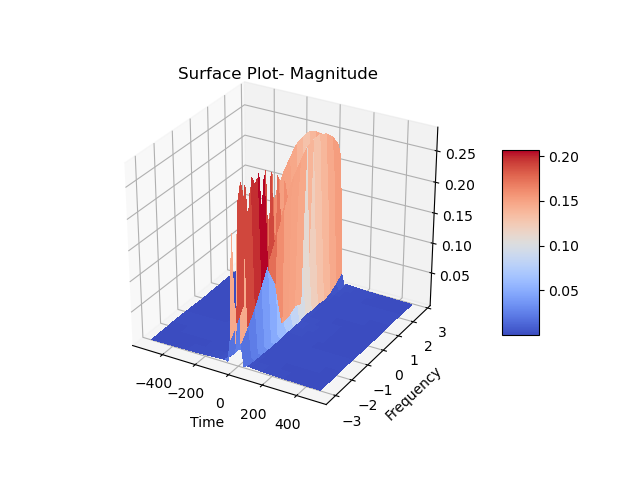
\includegraphics[scale=0.7]{Q6c.png}
	\caption{Magnitude Surface plot of the Chirped Signal without windowing}
 \end{figure} 

   \begin{figure}[!tbh]
   	\centering
   	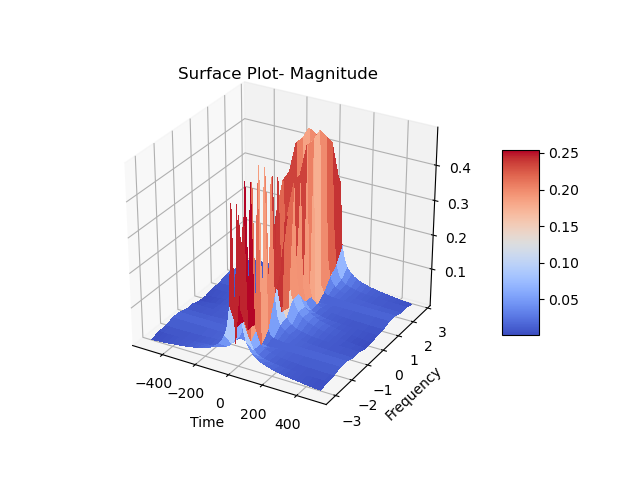
\includegraphics[scale=0.7]{Q6a.png}
	\caption{Magnitude Surface plot of the Chirped Signal}
 \end{figure} 

 
    \begin{figure}[!tbh]
   	\centering
   	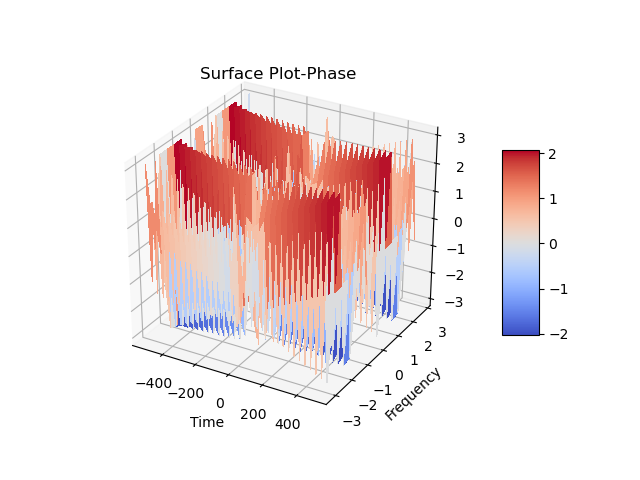
\includegraphics[scale=0.7]{Q6b.png}
	\caption{Phase Surface plot of the Chirped Signal}
 \end{figure} 
 
 \section*{Conclusions}
 \begin{itemize}
 \item In this assignment we have understood how important windowing is while plotting DFTs.We explored DFT without and with windowing. Windowing is used to make the signal integrable and it reduces the discontinuities in the actual signal that can lead to inaccurate DFTs .
 \item Hamming is to nullify the effect of Gibbs phenomena owing to the discontinuous nature of the series realised by a discrete fourier transform.
 \item  For a chirped signal, we plot fourier spectra for different time slices of a signal. We took closely spaced slices to get more intuition 
 \item In time varying plots some things are clearly observable like
\begin{itemize}
\item Existence of two peaks
\item Vanishing of chirp effects in windowed transform
\end{itemize}
 \end{itemize}  
\end{document}




